\documentclass[14pt]{article}
\usepackage[utf8]{inputenc}
\usepackage{tikz}
\usepackage{pgfplots}

\begin{document}
\LARGE

\section*{RETA}
\begin{tikzpicture}
 \draw (0,0) -- (6,0);
  \coordinate [label=left:A] (A) at (0,0);
  \coordinate [label=right:B] (B) at (6,0);  
   \draw (A) -- (B);
\end{tikzpicture}

\begin{tikzpicture}
   \coordinate [label=left:A] (A) at (0,0);
  \coordinate [label=right:B] (B) at (6,6);  
   \draw (A) -- (B);
\end{tikzpicture}

\section*{TRIÂNGULO}
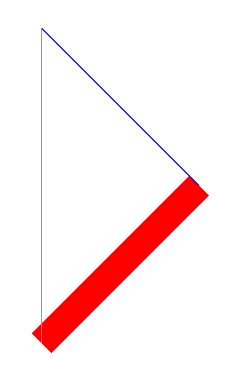
\begin{tikzpicture}
\draw[line width=10pt, red] (0,0) -- (2,2);
\draw[blue] (2,2) -- (0,4);
\draw[green] (0,4) -- (0,0);
\end{tikzpicture}

\section*{QUADRADO}
\begin{tikzpicture}
\draw (0,0) rectangle(4,4);
\end{tikzpicture}

\section*{RETÂNGULO}
\begin{tikzpicture}
\draw (0,0) rectangle(4,6);
\end{tikzpicture}

\vspace{2cm}

\begin{tikzpicture}
\draw (0,0) rectangle(6,4);
\end{tikzpicture}

\section*{CÍRCULO}

\begin{tikzpicture}
\draw[line width=2pt, blue] circle(2cm);
\end{tikzpicture}

\begin{tikzpicture}
\draw[line width=2pt, red] circle(10cm);
\end{tikzpicture}

\section*{ARCO}
\begin{tikzpicture}
\draw (0,0) arc(180:0:6);
\end{tikzpicture}

\section*{PLOTANDO GRÁFICOS}
\subsection*{FUNÇÃO}
\begin{tikzpicture}
%Montar o Plano cartesiano
\draw[line width=2pt,->] (-7,0) -- (7,0);
\draw[line width=2pt,->] (0,-7) -- (0,7);
%Plotar uma função
\draw[red] plot(\x,{2*cos(\x r)});
\end{tikzpicture}


\begin{tikzpicture}
 \begin{axis}[width=400pt,axis x line=middle, axis y line=center, tick align=outside]
 \addplot+[mark=none] (\x,{4*sin(\x r)});
 \end{axis}
\end{tikzpicture}


\begin{tikzpicture}
 \begin{axis}[width=400pt,axis x line=middle, axis y line=center, tick align=outside]
 \addplot+[mark=none] (\x,{ln(\x r)});
 \end{axis}
\end{tikzpicture}













\end{document}
